\documentclass{beamer}
\usepackage{fontspec}
\usepackage{xunicode}
\usepackage{xltxtra}
\usepackage{xecyr}
\usepackage{hyperref}
\setmainfont[Mapping=tex-text]{DejaVu Serif}
\setsansfont[Mapping=tex-text]{DejaVu Sans}
\setmonofont[Mapping=tex-text]{DejaVu Sans Mono}
\usepackage{polyglossia}
\setdefaultlanguage{russian}
\setotherlanguage{english}
\usepackage{graphicx}
\usepackage{listings}
\lstdefinestyle{mycode}{
  belowcaptionskip=1\baselineskip,
  breaklines=true,
  xleftmargin=\parindent,
  showstringspaces=false,
  basicstyle=\footnotesize\ttfamily,
  keywordstyle=\bfseries,
  commentstyle=\itshape\color{gray!40!black},
  stringstyle=\color{red},
  numbers=left,
  numbersep=5pt,
  numberstyle=\tiny\color{gray},
}
\lstset{escapechar=@,style=mycode}

\newcommand{\cimg}[2]{%
	\begin{center}%
		\ifthenelse{\equal{#2}{}}{%
			\includegraphics[width=0.75\linewidth]{#1}
		}{%
			\includegraphics[width=#2\linewidth]{#1}
		}%
	\end{center}%
}

\usetheme{Antibes}
\useoutertheme{infolines}

\title{Curse Words Detector}
\subtitle{project}
\author{Беляев Станислав}
\institute{СПб АУ РАН}
\date{Весна 2016}

\setbeamercovered{highly dynamic}
\newcounter{saveenumi}
\newcommand{\seti}{\setcounter{saveenumi}{\value{enumi}}}
\newcommand{\conti}{\setcounter{enumi}{\value{saveenumi}}}

\begin{document}

\frame{\titlepage}

\section{Цели и задачи}
\begin{frame}[<+->]{Цели и задачи}
    \begin{enumerate}
        \item Модуль на питоне для блокировки слов
        \item Тесты
        \item Профиллирование работы
        \item Поместить это внутрь Node.js
    \end{enumerate}
\end{frame}

\section{Архитектура проекта}
\begin{frame}[t]{Архитектура проекта}
    Дано слово $w$, нужно найти ближайшее к нему "плохое" $c$
    $$argmax_c ~ {P(c|w)} = argmax_c ~ {P(w|c) \frac{P(c)}{P(w)}}$$
    \begin{enumerate}
        \item $P(c)$ - "how likely is c to appear in text?"
            \begin{itemize}
                \item частотные списки взял у opencorpora
            \end{itemize}
        \item $P(w)$ - "same for every c"
        \item $P(w|c)$ - вероятность того, что автор написал $w$, подразумевая $c$
            \begin{itemize}
                \item edit distance $\leqslant 2$
            \end{itemize}
        \item $argmax_c$ - максимум по всем $c$
    \end{enumerate}
\end{frame}
\begin{frame}[t]{Архитектура проекта}
    Модули на python3:
    \begin{enumerate}
        \item Purifier - main
        \item Analizier - работа с нормальной формой + предиктор
        \item Heurister - эвристическая замена цифр и латинских букв на русские
        \item Statisticer $\&$ Tester - классы для сбора статистики и тестов
    \end{enumerate}
\end{frame}

\section{Результаты}
\begin{frame}[t]{Результаты}
    \begin{center}
        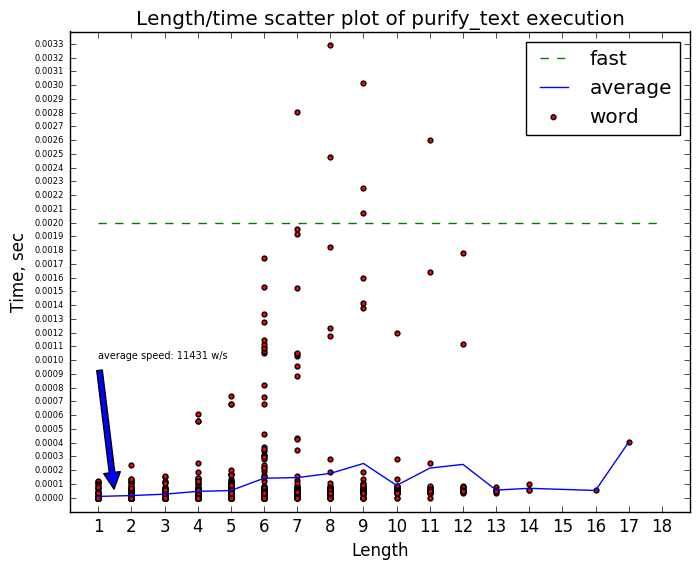
\includegraphics[width=0.74\linewidth]{length_time_plot.png}
    \end{center}
\end{frame}

\section{Конец}
\begin{frame}[t]{Конец}
    \begin{center}
    Спасибо за внимание
    \end{center}
	\begin{description}
		\item[GitHub:]  \url{https://github.com/StasBel/CurseWordsDetector}
	\end{description}
\end{frame}

\end{document}